% !TeX encoding = UTF-8
\documentclass[12pt]{report}
\usepackage[utf8]{inputenc}
\usepackage[T1]{fontenc}
\usepackage[english]{babel}
\usepackage{graphicx}
\usepackage{titlesec}
\usepackage{hyperref}
\hypersetup{
  colorlinks=true,
  linkcolor=blue,
  urlcolor=blue,
  linktoc=all
}
\graphicspath{{images/}}
\titleformat{\chapter}[hang]{\normalfont\huge\bfseries}{\thechapter.}{1em}{}

\title{Torque Vectoring}
\author{}
\date{\today}

\begin{document}

\setcounter{secnumdepth}{3}

\maketitle

\tableofcontents

\cleardoublepage

\chapter{Introduction}
\label{chap:introduction}

Torque vectoring is a widely known technique to improve vehicle handling and to increase stability in limit conditions. With the advent of electric vehicles, this is becoming a key topic since it is possible to have distributed powertrains. The possibility of independently controlling the torque on each wheel quickly and precisely makes applying Torque Vectoring Control (TVC) strategies easy. Indeed, Torque Vectoring (TV) consists in applying different longitudinal forces to the wheels of the same axle, resulting in a yaw moment that is used to control the vehicle lateral dynamics.

Regarding TV control architecture, most of the literature proposes a multilayer cascaded control composed by three main blocks, as in Figure~\ref{fig:tv_control_scheme}, which include the following:
\begin{itemize}
  \item reference generator;
  \item high-level controller;
  \item low-level controller.
\end{itemize}

\IfFileExists{Images/TV_control_scheme.png}{%
  \begin{figure}[htbp]
    \centering
    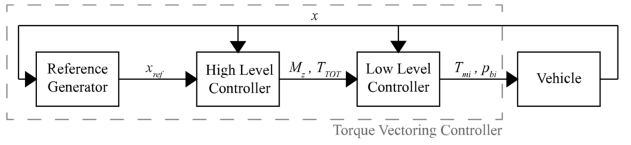
\includegraphics[width=0.8\textwidth]{Images/TV_control_scheme.png}
    \caption{TV control scheme}
    \label{fig:tv_control_scheme}
  \end{figure}
}{%
  \begin{figure}[htbp]
    \centering
    \fbox{\parbox{0.8\textwidth}{\centering [TV_control_scheme.png not found — add the image file to the `Images` folder]}}
    \caption{TV control scheme (placeholder)}
    \label{fig:tv_control_scheme_placeholder}
  \end{figure}
}

\section{V-Model design}
\label{sec:vmodel}

A V-model design was adopted for the development of the TVC system. 
As shown in Figure~\ref{fig:vmodel}, the left side of the V represents the decomposition of system requirements into more detailed specifications and design, while the right side represents the integration and verification of the system against those requirements.
The goal of adopting this model is to make the control architecture more scalable over time, providing a structure in which the control scheme can be improved and extended more easily in the future.


\IfFileExists{Images/V-model.jpg}{%
  \begin{figure}[htbp]
    \centering
    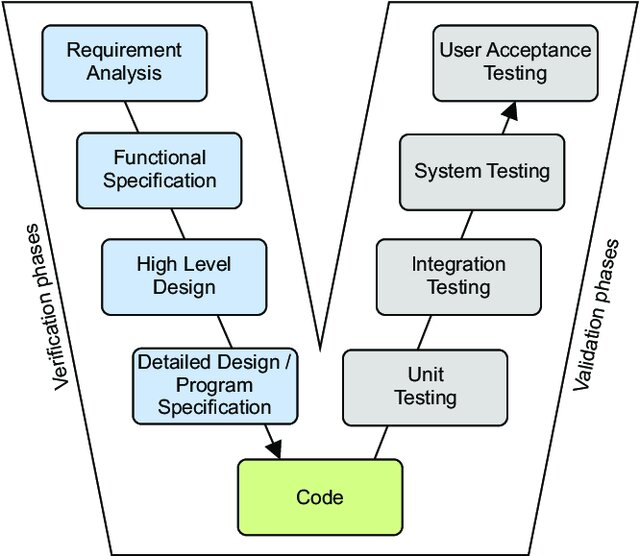
\includegraphics[width=0.8\textwidth]{Images/V-model.jpg}
    \caption{V-Model}
    \label{fig:vmodel}
  \end{figure}
}{%
  \begin{figure}[htbp]
    \centering
    \fbox{\parbox{0.8\textwidth}{\centering [V-model.jpg not found — add the image file to the `Images` folder]}}
    \caption{V-Model (placeholder)}
    \label{fig:vmodel_placeholder}
  \end{figure}
}

\section{Torque Vectoring Objectives}
\label{sec:tv_objectives}

The objectives of the implementation of a TVC system are the following:

\begin{itemize}
  \item \textbf{Handling Improvement:} Optimize turn-in and cornering performance. The system aims to make the vehicle track an ideal yaw rate computed by a reference model (Reference Generator), making steering response more reactive and compensating for chassis limitations.

  \item \textbf{Understeer Reduction:} Racing vehicles may exhibit a natural understeer gradient or one induced by load transfers. By providing driving torque to the outer wheel and braking (regenerative) torque to the inner wheel, TV generates a yaw moment in the same direction as the turn, actively counteracting the tendency of the car to run wide and helping to tighten the steering line.

  \item \textbf{Increased Stability in Limit Conditions:} During high-dynamic transient maneuvers, tires can quickly reach saturation (grip limit). TV, supported by an Anti-Skid (ASC) system, acts to promptly damp yaw-rate overshoot, preventing uncontrollable oversteer (spin) and keeping the vehicle on the trajectory desired by the driver.

  \item \textbf{Optimal Exploitation of the Electric Powertrain:} Leverage the fast response of inverters and the ability to manage regenerative braking in a corner to modulate vehicle attitude in real time, a dynamic advantage not achievable with a traditional passive mechanical differential.
\end{itemize}

\chapter{Requirement Analysis and System Constraints}
\label{chap:requirement_analysis}

In accordance with the first descending phase of the V-Model, the design of the Torque Vectoring Control (TVC) requires a preliminary and rigorous analysis of system requirements. For the controller to be stable and effective, it is necessary to define the physical, dynamic, and regulatory boundaries within which the vehicle operates. These constraints can be divided into two macro-categories: grip limits related to vehicle dynamics and electromechanical limitations of the powertrain.

\section{Vehicle Dynamics Limits and Tire Saturation}
\label{sec:vehicle_dynamics_limits}

The ideal yaw-rate reference generated for the controller is based on a linear single-track model. Although this model accurately describes vehicle behavior in linear conditions, it does not account for the decay of lateral tire forces at high slip angles.

To prevent the controller from requesting physically infeasible maneuvers (which would cause instability and trigger invasive Anti-Skid intervention), the following dynamic requirements were defined:

\begin{itemize}
  \item \textbf{Lateral Acceleration Saturation:} The maximum lateral acceleration tolerable by the vehicle is strictly constrained by the estimated friction coefficient ($\mu$) and gravitational acceleration ($g$). The Reference Generator must include dynamic saturation so that the reference yaw rate never exceeds the physical limit $r_{\max} = \frac{\mu \cdot g}{v_x}$.

  \item \textbf{Maneuver Targets:} The system must guarantee stability and responsiveness in maneuvers typical of Formula SAE tracks, which can include minimum curvature radii down to 4.5--5 m. This requires the system to handle large steering-wheel angles (up to and above 40 degrees) while keeping the vehicle in its maximum lateral-performance region.

  \item \textbf{Understeer Gradient:} The chassis exhibits a natural understeer gradient that depends on static mass distribution and front/rear axle cornering stiffness. The TVC must generate a compensating yaw moment capable of canceling or mitigating the vehicle's intrinsic understeering/oversteering component, enforcing a predominantly neutral behavior.
\end{itemize}

\section{Powertrain Constraints and Actuation Limits}
\label{sec:powertrain_constraints}

Torque distribution strategies (Low-Level Controller or Torque Allocator) must strictly comply with the hardware specifications of the electric motors and inverters. Nominal parameters extracted from vehicle analysis impose the following actuation constraints:

\begin{itemize}
  \item \textbf{Maximum Drive Torque (Traction):} Each individual motor can deliver a maximum positive torque of $T_{drive,\max} = 400\,\mathrm{Nm}$.

  \item \textbf{Maximum Braking Torque (Regenerative):} The regenerative torque limit absorbable by the inverter and battery pack is limited to $T_{regen,\max} = -25\,\mathrm{Nm}$ . This limit introduces strong actuation asymmetry: the TV capability to brake the inner wheel is significantly lower than its capability to push the outer wheel. The controller must be tuned to prevent integral-action wind-up when this limit is reached prematurely.
\end{itemize}

The identification of these limits provides the foundation for the subsequent design phases (High-Level Design), justifying the need to implement Anti-Windup logic in the PID and an Anti-Skid (ASC) system to manage grip losses caused by torque transients.

\chapter{System Architecture and Detailed Design}
\label{chap:system_architecture}

This chapter illustrates the logical architecture and the mathematical implementation of the Torque Vectoring Control (TVC) system. The controller design was developed following a modular top-down approach, allowing each component of the control chain to be isolated and validated individually.

\section{Control Layout and Reference Scheme}
\label{sec:control_layout_reference_scheme}

As anticipated in the general scheme in Chapter~1 and shown in \hyperref[fig:tv_control_scheme]{Figure~\ref*{fig:tv_control_scheme}}, the architecture is based on a cascaded-loop structure. The driver input (steering angle and torque request) and vehicle state (speed, yaw rate) are processed sequentially by three macro-blocks:

\begin{enumerate}
  \item \textbf{Reference Generator:} Computes the ideal dynamic target.
  \item \textbf{High-Level Controller:} Computes the corrective yaw moment ($M_z$).
  \item \textbf{Low-Level Controller (Torque Allocator):} Distributes physical torque to the wheels.
\end{enumerate}

\section{Reference Generator}
\label{sec:reference_generator}

The reference generator is the dynamic brain of the system. Its task is to translate the driver's intent into a target yaw rate ($\dot{\psi}_{ref}$).

The computation is based on the linear kinematic bicycle model, which depends on longitudinal speed ($v_x$), wheel steering angle ($\delta$), and the chassis understeer gradient ($K_{us}$):

\[
\dot{\psi}_{linear} = \frac{v_x \cdot \delta}{L + K_{us} \cdot v_x^2}
\]

The linear model assumes infinite tire grip, which is an unacceptable approximation in limit driving. To prevent the controller from requesting physically infeasible cornering, the signal is passed through a dynamic saturator based on the maximum tolerable lateral acceleration ($a_y = \mu \cdot g$). The final reference is therefore limited to:

\[
\dot{\psi}_{max} = \frac{\mu \cdot g}{v_x}
\]

If $\dot{\psi}_{linear}$ exceeds this limit, the system outputs $\dot{\psi}_{max}$, ensuring that targets remain within the friction ellipse.

\section{High-Level Controller (Yaw Rate Control)}
\label{sec:high_level_controller}

The high-level controller has the task of nullifying the error between the desired yaw rate and the actual yaw rate measured by the IMU: $e = \dot{\psi}_{ref} - \dot{\psi}_{real}$.

\subsection{Fujimoto Scheme}
\label{subsec:fujimoto_scheme}

The basic architecture is strongly inspired by the control scheme proposed by Fujimoto, as shown in Figure~\ref{fig:fujimoto_scheme}.

\IfFileExists{Images/fujimoto.jpeg}{%
  \begin{figure}[htbp]
    \centering
    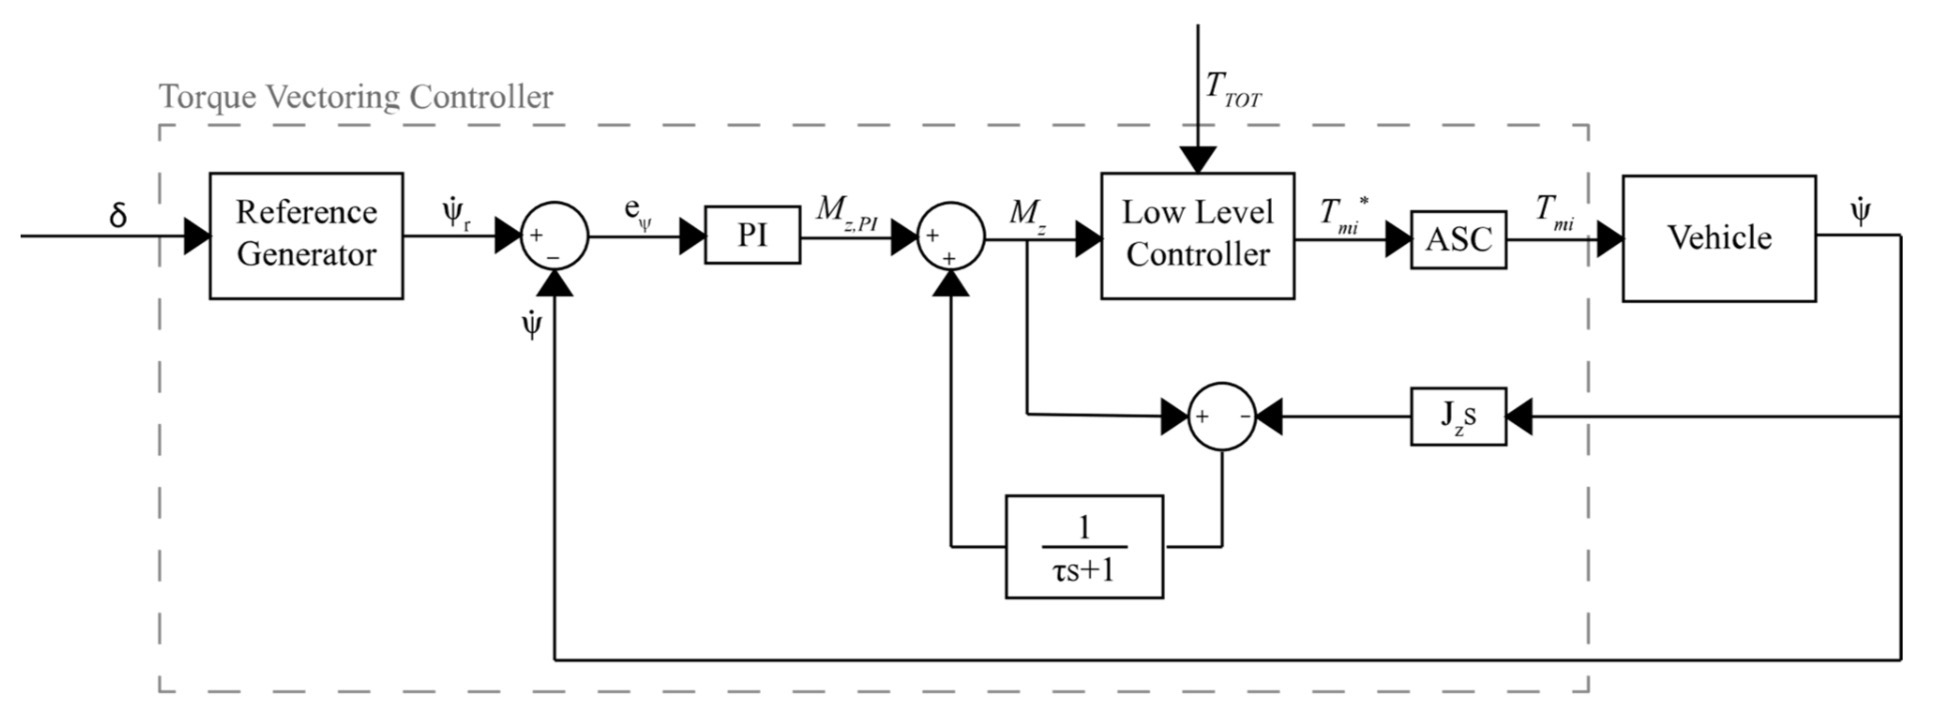
\includegraphics[width=0.8\textwidth]{Images/fujimoto.jpeg}
    \caption{Fujimoto control scheme}
    \label{fig:fujimoto_scheme}
  \end{figure}
}{%
  \begin{figure}[htbp]
    \centering
    \fbox{\parbox{0.8\textwidth}{\centering [fujimoto.jpeg not found — add the image file to the `Images` folder]}}
    \caption{Fujimoto control scheme (placeholder)}
    \label{fig:fujimoto_scheme_placeholder}
  \end{figure}
}

This scheme employs a PI controller coupled with a Disturbance Observer (DOB) based on the derivative of the yaw rate, useful for rejecting external disturbances not predicted by the model (e.g., asymmetric grip variations) and includes cascaded Anti-Skid Control integration.

\subsubsection{DOB Behavior and Simplification Strategy}
\label{subsubsec:dob_behavior}

During initial transient simulation phases, the high initial angular acceleration saturated the DOB, injecting a counteracting reaction that destabilized the vehicle. Adopting an iterative development approach, it was decided to temporarily exclude the Disturbance Observer branch, entrusting control to the PI loop alone. This configuration guarantees high baseline robustness, leaving the reintroduction of the DOB to future developments and tuning.

\subsection{PI: Gain Scheduling}
\label{subsec:pi_gain_scheduling}

Although the Proportional-Integral (PI) controller structure is standard, the vehicle lateral dynamics are strongly nonlinear and vary significantly with longitudinal speed. A controller tuned with fixed gains for high speeds would be too sluggish at low speeds, while one tuned for low speeds would make the vehicle unstable in fast sections.

To solve this problem, a Gain Scheduling strategy was implemented. The parameter computation procedure was based on the study of the poles of the linearized system. The dynamic analysis showed that, especially at low speeds, the vehicle exhibits ``slow'' poles that make the system response sluggish and poorly reactive.

To maximize performance, the integral gain ($K_i$) was computed analytically for each operating point with the goal of cancelling the slow pole of the system. This synthesis technique makes it possible to replace the natural vehicle dynamics with a much faster closed-loop response, while maintaining a constant damping ratio over the entire speed range.

The results of this study, carried out in MATLAB, were exported to a Look-Up Table (LUT). During execution on the VCU, the controller reads the current longitudinal speed and linearly interpolates the table values, dynamically updating the $K_i$ value. This ensures that the controlled system always maintains the same response readiness and stability, regardless of driving speed.

\subsubsection{LUT Details}
\label{subsubsec:lut_details}

The Gain Scheduling map was generated for longitudinal speeds from $1\,\mathrm{m/s}$ to $30\,\mathrm{m/s}$, using a uniform step of $1\,\mathrm{m/s}$. This discretization provides a dense and regular grid of operating points, enabling stable linear interpolation of $K_i$ during real-time execution on the VCU.

Table~\ref{tab:ki_lut_last5} reports an example subset of the implemented LUT, showing the last five speed entries and their corresponding integral gains.

\begin{table}[htbp]
  \centering
  \caption{Example of last five entries of the implemented $K_i$ LUT}
  \label{tab:ki_lut_last5}
  \begin{tabular}{cc}
    \hline
    $V_x$ [m/s] & $K_i$ [-] \\
    \hline
    26 & 15595.7 \\
    27 & 14208.8 \\
    28 & 12913.8 \\
    29 & 11701.9 \\
    30 & 10565.0 \\
    \hline
  \end{tabular}
\end{table}

\subsection{Anti-Windup (Clamping)}
\label{subsec:anti_windup}

Due to the thermal and mechanical asymmetry of the powertrain (traction capability of $+400\,\mathrm{Nm}$ against a much lower regenerative peak limit), actuators can saturate rapidly during aggressive cornering. To prevent wind-up phenomena (uncontrolled accumulation of integral action while motors are at their limit), an Anti-Windup system of Clamping type has been implemented.

The system computes the maximum yaw moment theoretically generatable by the rear motors ($M_{z,\max}$); if the PI request exceeds this limit and the error has the same sign, the integral accumulator is temporarily frozen until returning to the linear region.

\end{document}
